\subsection{RLC en serie}\label{sec:RLC serie}
\paragraph{}En esta sección, se estudió la respuesta de un circuito RLC en serie y, en particular, su resonancia. Para esto, se armó el circuito de la figura \ref{fig:RLC-SERIE}, que consiste de una fuente de tensión alterna, un resistor, un inductor y un capacitor conectados en serie. 


\begin{figure} [H]
    \centering
    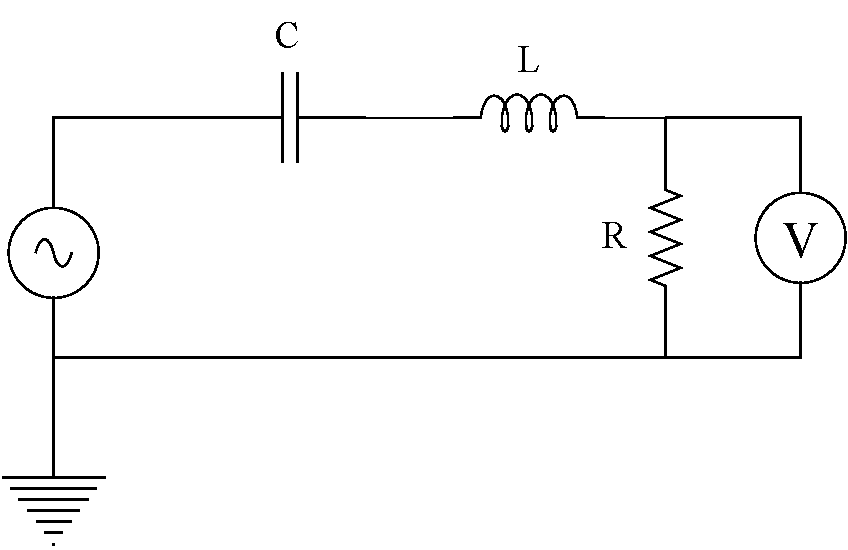
\includegraphics[width = 0.6\linewidth]{Esquemas/RLC-SERIE.drawio.pdf}
    \caption{Esquema que representa el circuito RLC en serie formado por una fuente de tensión alterna, una resistencia $R$, una capacitancia $C$ y una inductancia $L$. Sumado a esto, se agrega un voltímetro que mide la caída de tensión en la resistencia.}
    \label{fig:RLC-SERIE}
\end{figure}

\paragraph{}
Se realizó un barrido de frecuencias y se registró la caída de tensión en $R$ y el defasaje para tres valores de $R$. El valor de $R$ modifica significativamente el ancho de la campana y, por lo tanto, el factor de mérito. Este registro se realizó con un osciloscopio, recolectando los datos para cada frecuencia directamente del dispositivo. Con estos datos, se realizó un ajuste para determinar la frecuencia y la tensión y, utilizando estos coeficientes con sus respectivos errores, se realizó un ajuste con la ecuación. Este procedimiento resultó en errores relativos muy bajos. En la figura se encuentran el gráfico la potencia disipada por la resistencia $R$, los diagramas de Bode del defasaje y la atenuación, todos en función de $\omega/\omega_{0}$, para el primer valor de resistencia.

\paragraph{} Se analizaron tres configuraciones para el RLC-serie con distintos valores de $R$ medidos aparte con un ohmetro. Se debe destacar que la resistencia total del sistema es una suma de las resistencias del resistor, inductor y fuente.



%-------------------POTENCIA--------------------vvvvvv
\paragraph{}Para el ajuste de la potencia se utilizó la ecuación (\ref{eq:corriente serie}).

\begin{figure} [H]
    \centering
    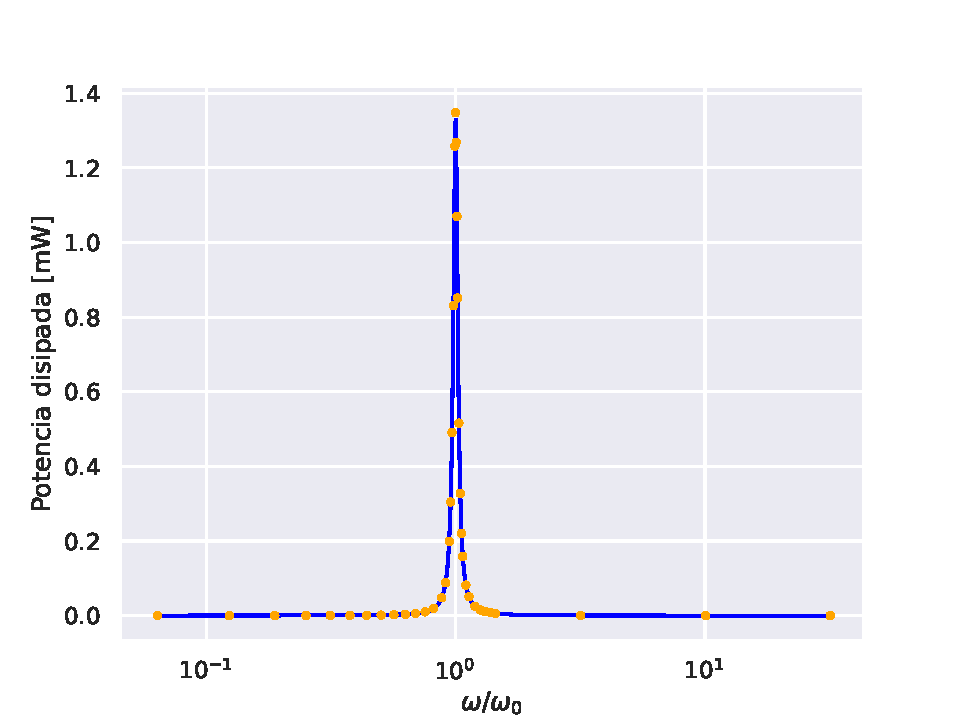
\includegraphics[scale=0.5]{figuras/RLC-SERIE-1/potencia.pdf}
    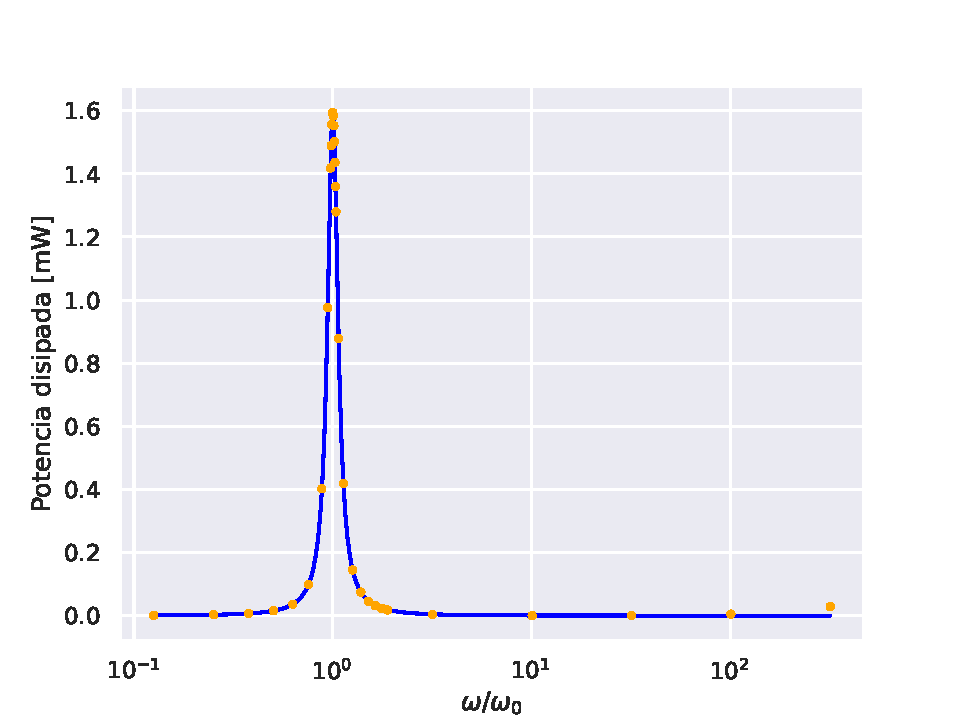
\includegraphics[scale=0.5]{figuras/RLC-SERIE-2/potencia.pdf}
    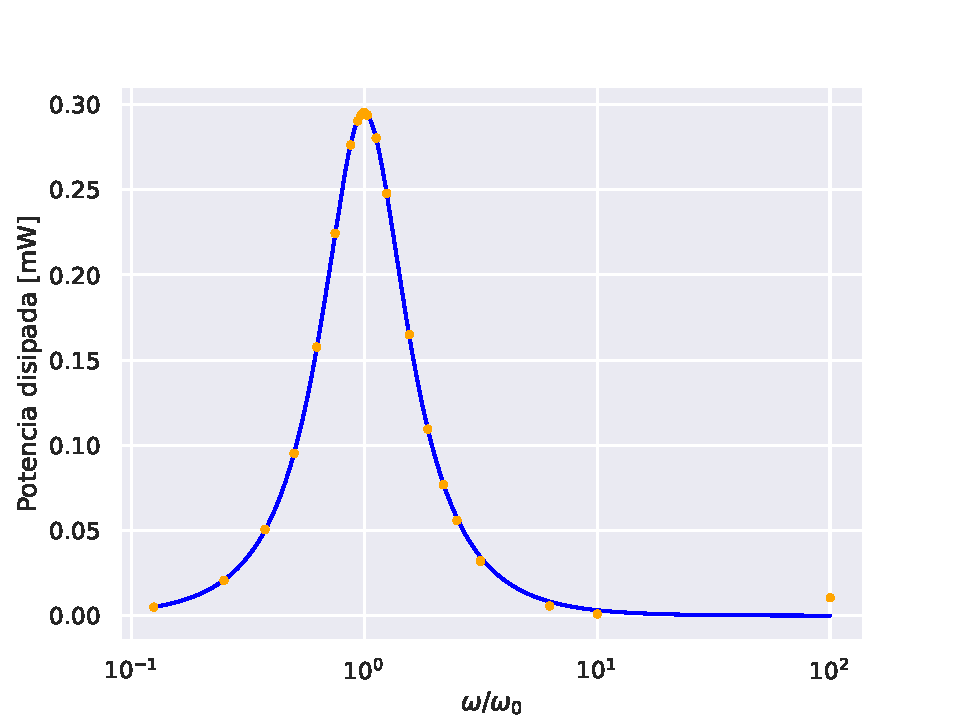
\includegraphics[scale=0.5]{figuras/RLC-SERIE-3/potencia.pdf}
    \caption{Gráfico de la potencia en función de $\frac{\omega}{\omega_0}$. Como puede apreciarse, la función aumenta hasta alcanzar un máximo en $f_0$ y luego comienza a descender. Este comportamiento es propio de un sistema resonante, donde la frecuencia de resonancia es aquella en la que la función alcanza su máximo. El $f_0$ de la configuración 2 y 3 coincide mayormente con el de la configuración 1. Sin embargo, se distinguen diferencias en el ancho de la campana de resonancia. A medida que se aumentó la reistencia, se obtuvieron campanas más anchas. Cabe destacar que por encima del orden de los $10^5$ Hz la curva de las configuraciones 2 y 3 ya no pasan por los puntos.}
    \label{fig:potencia_serie}
\end{figure}

\paragraph{} Para la primera configuración se utilizó una resistencia de $(R=151 \pm 1)\ \Omega$. 
Se obtuvo un $f_0 = (1590.22 \pm 0.03)$ Hz. Se obtuvo un factor de mérito de  $Q_1= 20.49 \pm 0.02$.

\paragraph{} Para la segunda configuración se usó una resistencia de $(R= 1151 \pm 1)\ \Omega$. Se obtuvo una resonancia en $f_0 = (1590.08 \pm 0.09)$ Hz, como puede verse en la figura \ref{fig:potencia_serie}. Este resultado es consistente, dado que no se varió ningún elemento del sistema que pueda afectar a $f_0$. El ancho de banda obtenido es de $Q_2 = (6.84 \pm 0.01)$. Esto es coherente dado que al aumentar la resistencia, la campana aumenta en ancho, por lo que su factor de mérito disminuye. Por encima del orden de los $10^5$ Hz el modelo no se ajusta correctamente a los datos, por lo que el modelo no es útil para frecuencias tan altas en esta configuración. 

\paragraph{}En la tercera configuración se usó una resistencia de $(R= 10151 \pm 1)\ \Omega$. el $f_0$ obtenido fue de $f_0 = (1597.62 \pm 0.61)$. El factor de mérito obtenido es de $Q_3 = 0.97 \pm 0.01$. 

\paragraph{} La campana de resonancia en los tres casos está ubicada sobre el mismo $f_0$. A medida que se aumentó la cantidad de resistencia, se observó un aumento en el ancho de la campana. El aumento de la resistencia, también se evidenció en la disminución en $Q$. Por encima del orden de los $10^5$ Hz y al igual que en el caso anterior, el modelo no se ajusta correctamente a los datos, por lo que no es útil para frecuencias tan altas en esta configuración. 

\paragraph{}Con este análisis se puede apreciar que la campana de resonancia aumentó en ancho a medida que se aumentaba $R$, reduciendo así su factor de mérito. La frecuencia de resonancia no sufrió cambios significativos con la variación de $R$. Las frecuencias de resonancia obtenidas son razonablemente similares, pero no exactamente, especialmente en el último caso. Por último, se debe tener en cuenta que el modelo utilizado presenta inconsistencias y estas se evidencian progresivamente con el aumento de $R$.




%---------------------DIAGRAMAS DE BODE---------------------vvvvvv

\paragraph{}
De estos mismos datos se obtuvo el gráfico de la figura que muestra la atenuación en función de $\frac{\omega}{\omega_0}$. Este ajuste se realizó por medio de la ecuación (\ref{eq:corriente serie}) en la ecuación (\ref{eq:atenuacion}).

\begin{figure} [H]
    \centering
    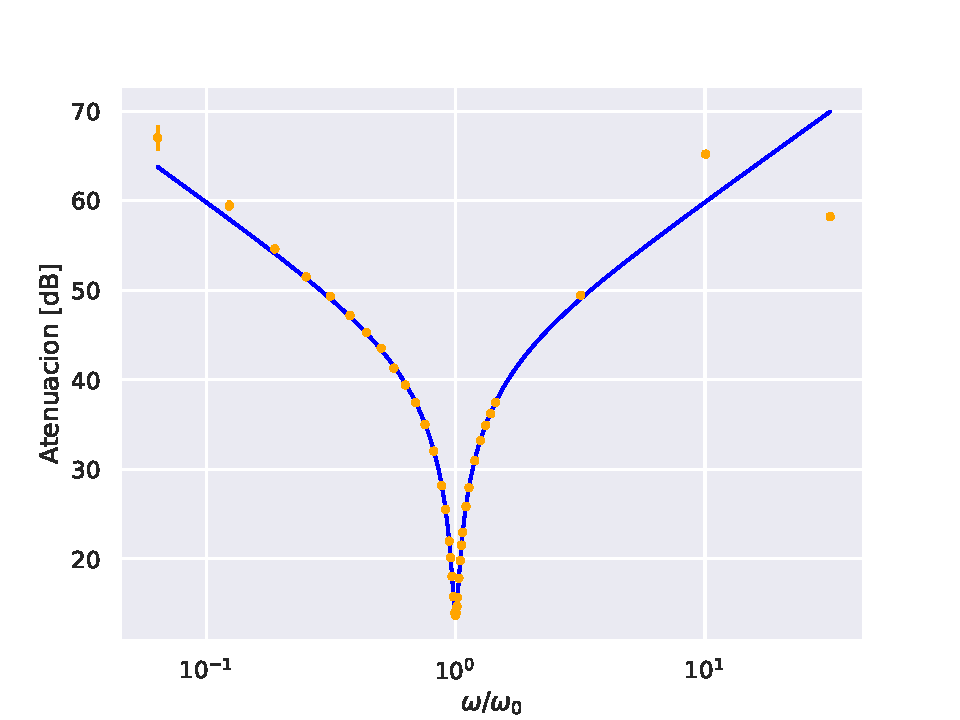
\includegraphics[scale=0.5]{figuras/RLC-SERIE-1/atenuacion.pdf}
    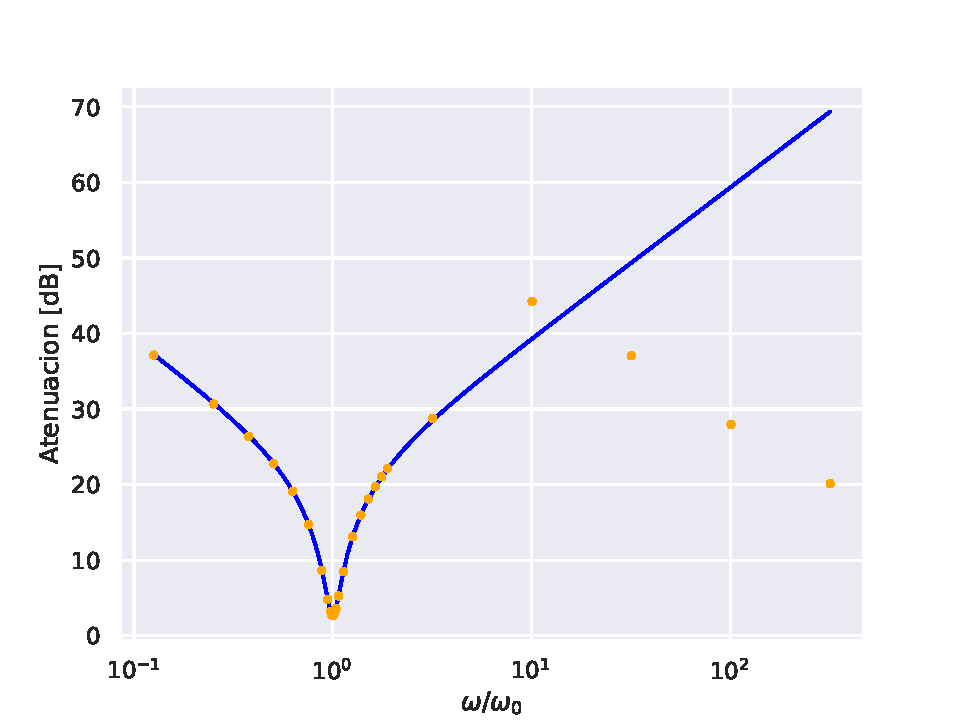
\includegraphics[scale=0.5]{figuras/RLC-SERIE-2/atenuacion.pdf}
    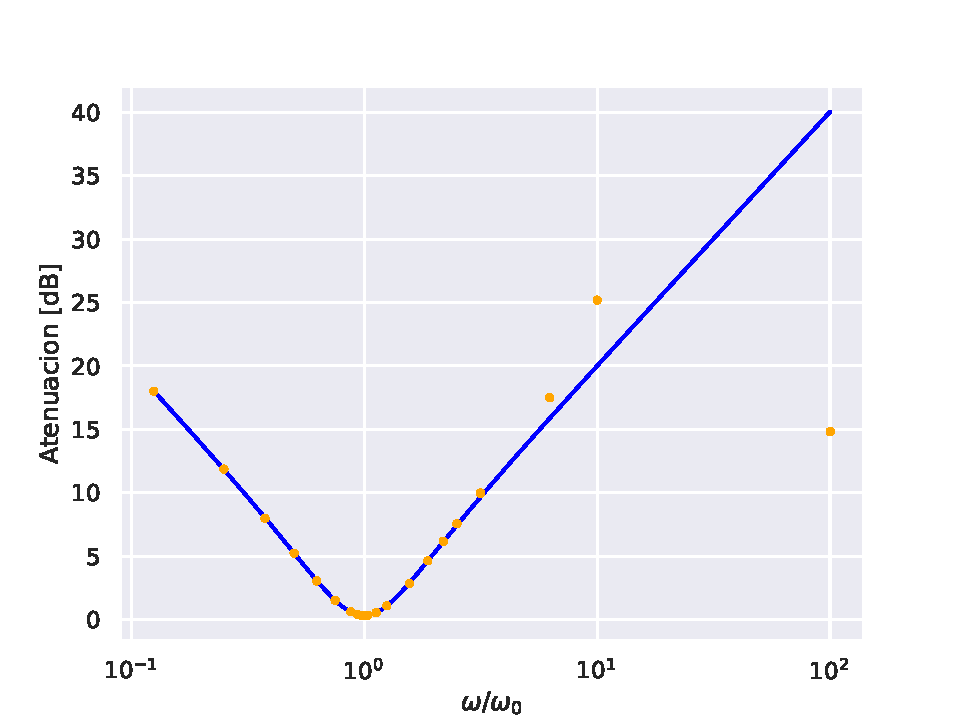
\includegraphics[scale=0.5]{figuras/RLC-SERIE-3/atenuacion.pdf}
    \caption{Se observa una disminución en la atenuación, un mínimo y a medida que se sigue aumentando la frecuencia, vuelve a aumentar la atenuación. En el orden de los MHz el modelo no se ajusta a los datos.}
    \label{fig:atenuación_serie}
\end{figure}


%---------------------atenuacion v w/w0---------------------vvvvvv



%----------------------------fase---------------------------vvvvvv

\paragraph{}
Para el desfasaje, se realizó un ajuste por la ecuación (\ref{eq:RLC-SERIE-PREDICCION-FASE}).


\begin{figure} [H]
    \centering
    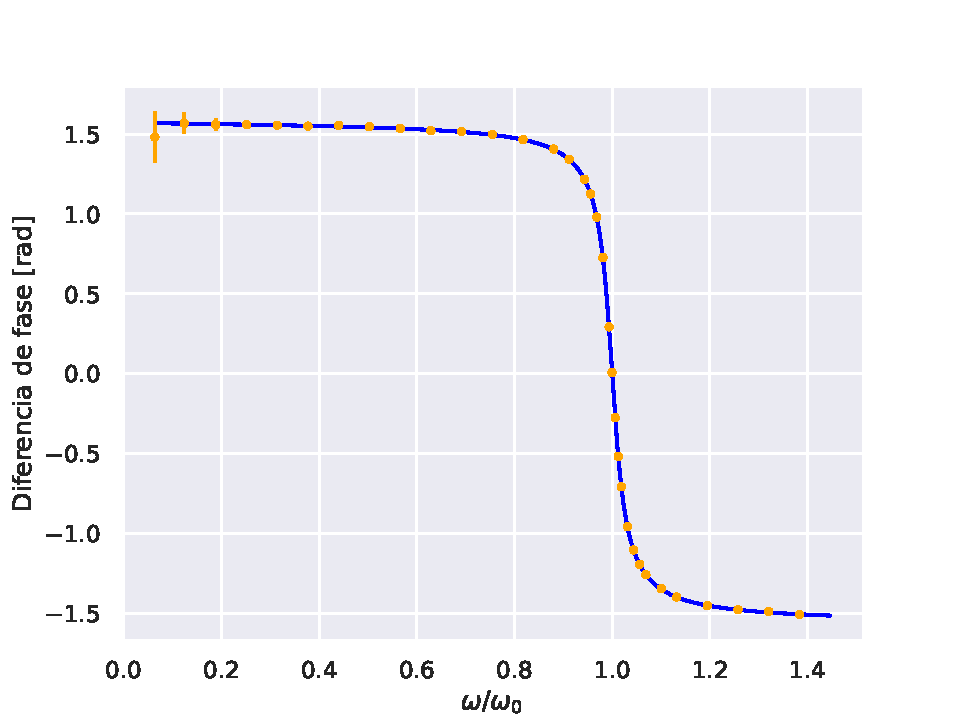
\includegraphics[scale=0.5]{figuras/RLC-SERIE-1/fase.pdf}
    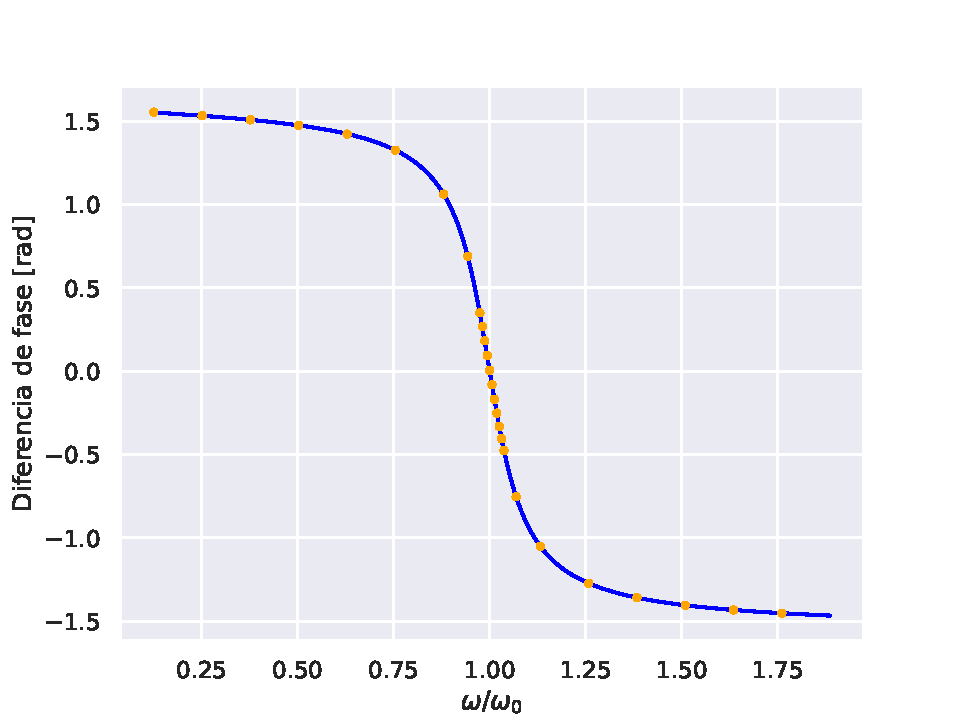
\includegraphics[scale=0.5]{figuras/RLC-SERIE-2/fase.pdf}
    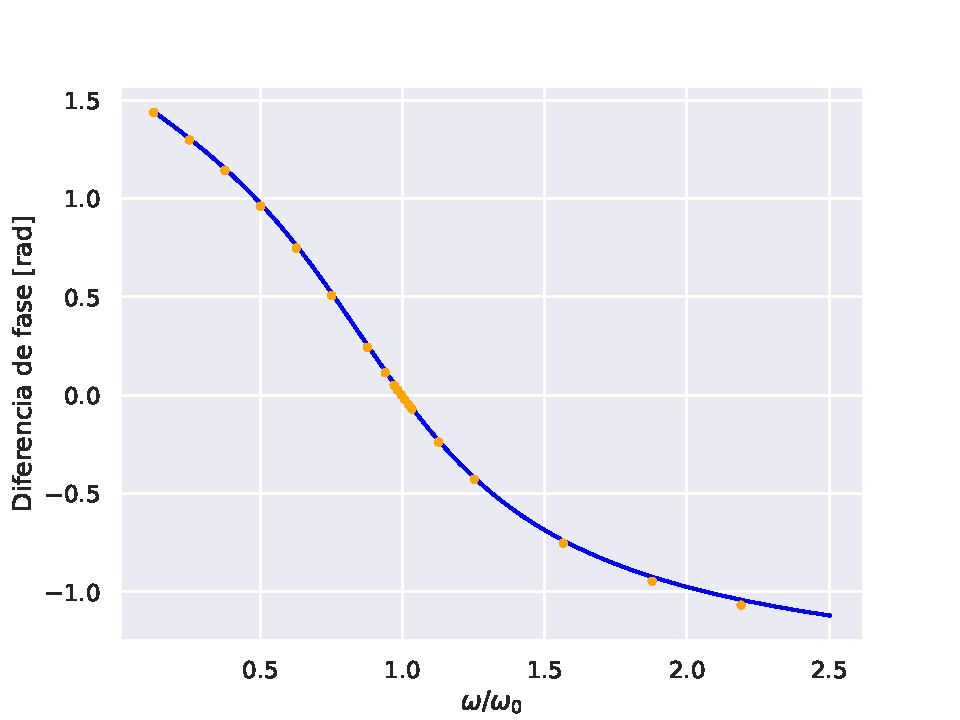
\includegraphics[scale=0.5]{figuras/RLC-SERIE-3/fase.pdf}
    \caption{Gráficos de la fase en función del cociente de $\omega$ Se muestran la diferencia de fase en función del cociente entre $\omega$ y $\omega_0$. Como puede verse el modelo se ajusta razonablemente a los datos.}
    \label{fig:fase_serie}
\end{figure}
